\subsection{Benchmarking for Employee Use Case}
(Maybe start text fancy with the questions which araise during the project: see the benchmarking google sheet for that)

As already mentioned this project was carried out as a prototyping project. Therefore we need to benchmark our results against the current best practice. Current state of the art for deploying contracts to the ethereum blockchain includes saving all the state variables of the contract on the blockchain and thus on all machines participating in the blockchain. As proposed we want to save those state variables off from the blockchain and thus save on gas which explains why gas cost are our most important measurement.

%- What did we benchmark?
%Explain which scenarios we did test (1 employee, multiple employee)
We especially benchmarked the employee use case as the employee use case is the more complex one of our both use cases. As a preparation for benchmarking we first needed two different smart contracts. One smart contract that works completely on-chain without using any external database, hashing functions or merkle trees and another smart contract that uses all introduced methods that are needed in order to off-chain our data to an external database. The two variants behave completely similar except for the saving of the state variables. Both variants are completely functional and could be used as they are if someone would like to deploy the employee use case. These fact were very important to us because only like that we could make sure that our benchmarks lead to meaningful results. Within the employee use case we measured different scenarios which will be described in the corresponding sections, mainly a time measure as well as a simple and another complex measure for the gas cost have been made.

%Explain under which aspects we did benchmark (gas, time)
%Mention again why gas is of utmost importance to us (because it translates to money and time)
%Explain the thing with benchmarking only the overhead due to automining of ganache
We mainly benchmarked the two measurements gas cost and time. Gas cost was the initial motivation for off-chaining as we assumed to save on gas cost when we off-chain the state variables. Gas cost translates to real currency as a participant of the blockchain either needs to buy Ether or help to mine blocks in order to receive Ether which is needed to pay the resulting gas cost of a transaction. The time was measured as we wanted to gain insights into how much overhead our application adds to a normal blockchain application. This was possible as our technology stack includes ganache which is capable of automatically mining new transactions into new blocks instantly so that we are able to measure only the overhead that our application introduces.

- Nice transition into showing our first graphics.

- Insert graphics / statistics

Explain what is visible

Explain what that does mean

- Ellaborate on conclusions and findings from this evaluation

What do all the statistics say? what do they mean to us?

When does Off-Chaining make sense?

Do we really save gas?

-> Conclude on that

\subsubsection{Time measurement}
First we will measure the introduced computation time of our middleware for executing different functions of the smart contract. The result can be seen in Figure \ref{fig:05_time}.

As we measured the computation time multiple times we decided to unite the results into a box plot chart. Thus we can see how the system behaves most of the times and single outliers can easily be identified.

Thats a box plot chart

Everything under 1 second -> not relevant, no further measurements

multiple transactions in increase-salary with increasing size but not really relevant, as every transaction needs to be mined fist anyways

We can see the times in Figure \ref{fig:05_time}.

\begin{figure}[!htb]
\centering
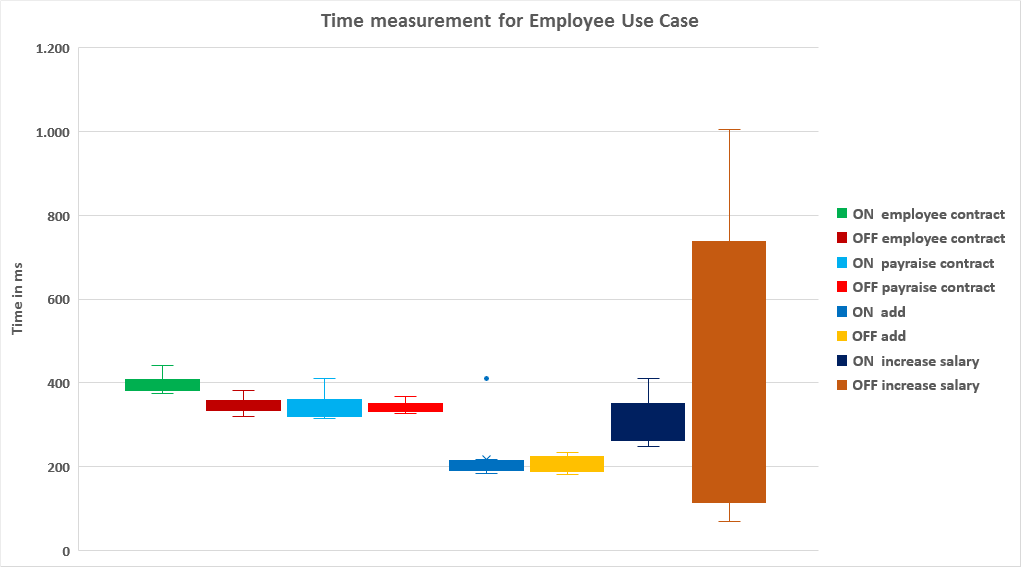
\includegraphics[width=1.0\textwidth]{images/05_time.png}
\caption{\label{fig:05_time}This are the times.}
\end{figure}


\subsubsection{Gas cost measurement}

And smth more in Figure \ref{fig:05_gas_cost_single}.

\begin{figure}[!htb]
\centering
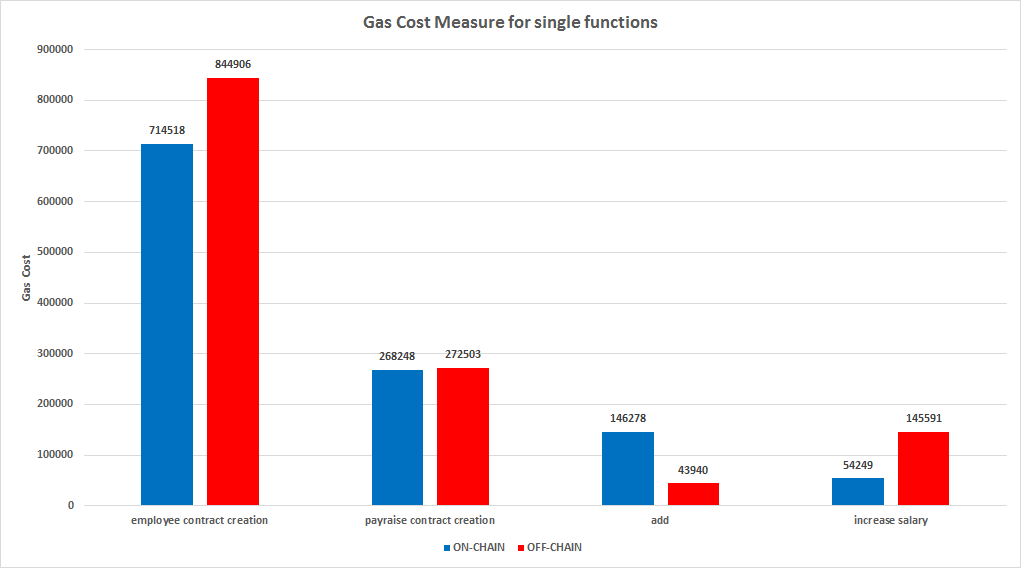
\includegraphics[width=1.0\textwidth]{images/05_gas_cost_single.png}
\caption{\label{fig:05_gas_cost_single}This is one employee.}
\end{figure}

And yet smth more in Figure \ref{fig:05_gas_cost_ten}.

\begin{figure}[!htb]
\centering
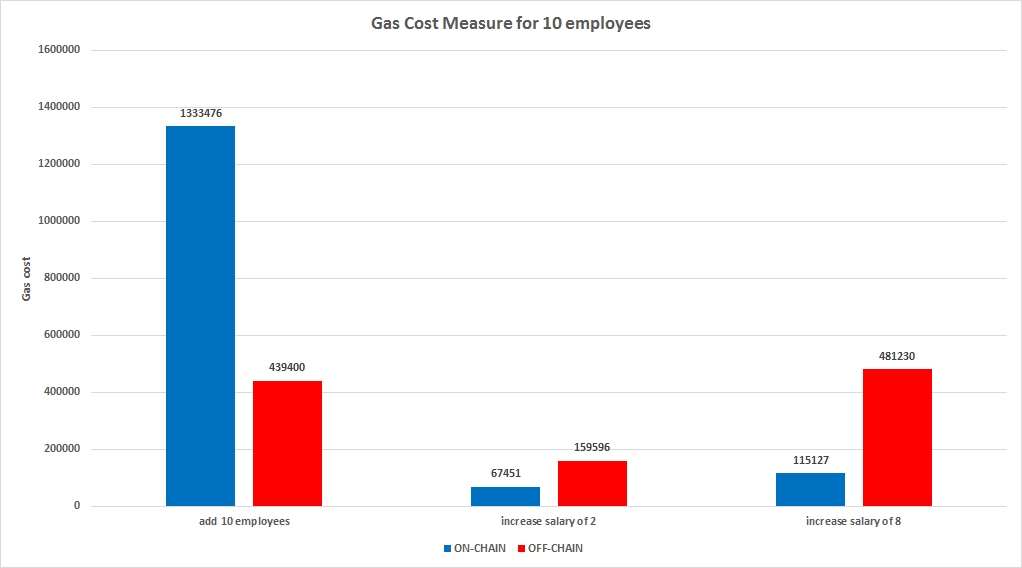
\includegraphics[width=1.0\textwidth]{images/05_gas_cost_ten.png}
\caption{\label{fig:05_gas_cost_ten}This is ten employees.}
\end{figure}